
\documentclass[
    a4paper,
    11pt
]{report}

\usepackage[utf8]{inputenc}

\usepackage{hyperref}
\usepackage{graphicx}

\usepackage{minted}
\usepackage{xcolor}

\newcommand{\Autor}{Felix Hirschel, Moritz Gutfleisch und Nico Thomas}
\author{Hirschel, Felix \and Gutfleisch, Moritz \and Thomas, Nico}
\newcommand{\MatrikelNummer}{4711}
\newcommand{\Kursbezeichnung}{Tinf19B1, Tinf19B4}

\newcommand{\Titel}{\LaTeX-Vorlage für diverse Ausarbeitungen\\--\\oder so ähnlich}
\newcommand{\AbgabeDatum}{1. April 2090}

\newcommand{\Dauer}{12 Wochen}

\newcommand{\Abschluss}{Bachelor of Science}

\newcommand{\Studiengang}{Informatik}

\newcommand{\Was}{Studienarbeit}

\hypersetup{%%
  pdfauthor={\Autor},
  pdftitle={\Titel},
  pdfsubject={\Was}
}


\begin{document}

\begin{titlepage}
\begin{center}
\vspace*{-2cm}
\FirmenLogoDeckblatt\hfill
\includegraphics[width=4cm]{dhbw-logo}\\[2cm]
{\Huge \Titel}\\[1cm]
{\Huge\scshape \Was}\\[1cm]
{\large für die Prüfung zum}\\[0.5cm]
{\Large \Abschluss}\\[0.5cm]
{\large des Studienganges \Studiengang}\\[0.5cm]
{\large an der}\\[0.5cm]
{\large Dualen Hochschule Baden-Württemberg Karlsruhe}\\[0.5cm]
{\large von}\\[0.5cm]
{\large\bfseries \Autor}\\[1cm]
{\large Abgabedatum \AbgabeDatum}
\vfill
\end{center}
\begin{tabular}{l@{\hspace{2cm}}l}
Bearbeitungszeitraum	         & \Dauer 			\\
Matrikelnummer	                 & \MatrikelNummer		\\
Kurs			         & \Kursbezeichnung		\\
Ausbildungsfirma	         & \FirmenName			\\
			         & \FirmenStadt			\\
Betreuer der Ausbildungsfirma	 & \BetreuerFirma		\\
Gutachter der Studienakademie	 & \BetreuerDHBW		\\
\end{tabular}
\end{titlepage}

\chapter{Einleitung}

Zu sagen Maschinensprache sei allgegenwärtig ist für nicht-Informatiker eine Aussage, mit der vermutlich zuerst nicht viel angefangen werden kann. Schließlich erfolgt der Kontakt mit den meisten elektronischen Geräten im Alltag entweder durch ein Touch Panel oder unterschiedliche Formen von Schaltern und Knöpfen, keine Eingabe von Nullen und Einsen. Wird sich länger mit der Thematik befasst, muss man feststellen, dass letzten Endes alle diese Interfaces nur eine Abstraktion darstellen. Keins steuert unmittelbar das Verhalten des darunterliegenden Systems insofern, dass ein System PC wüsste, was bspw. \glqq drucke Dokument\grqq{} bedeutet.

Damit Steuerungsanweisungen für elektronische Systeme verständlich werden, müssen diese in Zahlen vorliegen und zusätzlich müssen diese Zahlen interpretiert werden können. Schließlich handelt es sich um keine natürliche Form der Information. Die Interpretation geschieht seither mithilfe einer \ac{CPU}. Diese ist dazu in der Lage numerische Daten in Befehle umzusetzen und ein System mittels der Belegung von Pins, an die eventuelle Ein- und Ausgabegeräte angeschlossen sind, zu steuern.

In der heutigen Zeit gibt es nur noch für wenige Entwickler den Bedarf direkt auf die \ac{CPU} zuzugreifen, höherlevelige Sprachen vereinfachen den Zugriff soweit, dass die Informationsdarstellung dem Menschen in den meisten Fällen verständlich bleibt. Um ein tieferes Verständnis von der grundlegenden Funktionsweise digitaler Systeme zu erhaletn, bietet es sich trotzdem an, einmal mit Assembler, der Sprache am nähesten an Maschinensprache, zu arbeiten.
\medskip

Durch die Leistung heutiger PCs ist zur Ausführung von Maschinencode (zu bspw. Lernzwecken) keine zusätzliche \ac{CPU} in Hardware mehr notwendig. Stattdessen lässt sich deren Verhalten, je nach benötigter Leistung des gewünschten Systems, mit modernen Prozessoren simulieren. Vorliegende Arbeit befasst sich mit eben dieser Simulation eines älteren Mikroprozessors, dem Intel 8080.

Die Wahl fiel deshalb auf den Intel 8080, weil dieser als \glqq Einsteigerprozessor\grqq{} bekannt ist, sich also einerseits für Entwickler eignet, die erste Berührpunkte mit der Entwicklung auf Systemebene suchen, andererseits für die, die sich nocht nicht in großem Maß mit der Emulation solcher Systeme befasst haben. Der Ruf rührt vor allem daher, dass eine umfangreiche Dokumentation vorhanden ist und es sich um ein 8-Bit-System handelt, das eine überschaubare Menge an Befehlen unterstützt. Die genaue Funktionsweise und Eigenheiten werden in Kapitel \ref{chap:basics:intel8080} näher ausgeführt.

Wie später im Kapitel \glqq Verwandte Arbeiten\grqq{} (\ref{chap:similar-work}) dargestellt, gibt es auf dem Gebiet der Emulation bereits eine Vielzahl von Arbeiten, umgesetzt in den verschiedensten digitalen Ökosystemen. Die Simulation ist vor allem unter dem Aspekt interessant, einen tieferen Einblick in die Funktionsweise solcher Systeme, die Vorreiter unserer heutigen Generation von PCs sind, zu erhalten. Deshalb soll nicht nur der Prozessor als solcher emuliert werden, es soll auch eine Oberfläche entwickelt werden, die dem Anwender den Systemzustand zeigt und es ermöglicht eigenen Assemblercode zu schreiben, der so nah am Maschinencode wie möglich ist. Ein systematischer Aufbau der kompletten Anwendung ist in Kapitel \ref{chap:design} zu finden. Auf diesem basiert der Schwerpunkt der Arbeit, die Implementierung in Kapitel \ref{chap:impl}.

\chapter{Analyse}

\section{Zielstellung}\label{goals}

Das Ziel ist es einen Emulator zu entwickeln, welcher die vollständige Intel 8080 Spezifikation\cite{datasheet} unterstützt. Dabei sind die zentralen Aspekte wie folgt:

\begin{itemize}
    \item Vollständige 8080 Assembly Unterstützung
    \item Simulierte Schnittstelle zu Ein-/Ausgabegeräten
    \item Korrekte Behandlung von Hardware-Interrupts
\end{itemize}



Außerdem soll ein entsprechendes Web-Frontend entwickelt werden, um den Emulator zu bedienen.
Dieses soll einen Editor beinhalten, um Assembly Programme zu schreiben, die Ausführung dieser Programme ermöglichen, den Zustand des Emulators während der Ausführung darstellen und Auswahl zwischen verschiedenen Peripherie-Geräten ermöglichen (Pixel-Display, Eingabefeld, o.ä.). 

Es soll sowohl möglich sein Schritt für Schritt durch ein Programm zu gehen, als auch das Programm automatisch laufen zu lassen.

\section{Beitrag}

Unser Beitrag ist \Emu, ein in Rust geschriebener Intel 8080 Emulator mit Web-Frontend. \Emu erfüllt die gestellten Ziele vollständig.

Dadurch, dass unser Emulator nach Web-Assembly kompiliert wird, läuft der Emulator naiv im Browser des Clienten. Durch eine explizit definierte Schnitstelle, kann der Emulator mittels JavaScript Code bedient werden.

Der Editor unterstützt Syntax-Highlighting und Code-Completion und verfügt über Knöpfe um Kompilation und Ausführung des Programmes zu ermöglichen.
Es gibt Anzeigen für den Zustand der CPU (Register, Flaggen, etc.), für den Arbeitsspeicher und für die Peripherie-Geräte.\\

In \cref{chap:design} wird unser Design für den Emulator, die API und das Frontend
erläutert. Darauf folgend werden in \cref{chap:impl}

\chapter{Design}\label{chap:design}

\section{Emulator}

\subsection{Zentrale Struktur}

\begin{listing}[ht]
\begin{minted}{rust}
    struct Emulator {
        pc: u16,
        sp: u16,
        ram: RAM,
        reg: RegisterArray,
        input_devices: [InputDevice; 256],
        output_devices: [OutputDevice; 256],
        running: bool,
        interrupts_enabled: bool
    }
\end{minted}
\centering
\caption{Zentrale Emulator Struktur}
\label{lst:wtf}
\end{listing}

Den Kern des Emulators bildet eine Struktur, welche zuständig für die Ausführung der Maschinencode-Programme ist. Diese Struktur gruppiert alle notwendigen Komponenten eines Intel 8080 Systems. Der Aufbau der Struktur ist in \cref{lst:wtf} illustriert.

Diese Komponenten wurden in \cref{chap:prereqs} bereits erklärt: \rust{pc} und \rust{sp} sind 2 16-Bit-Zahlen, die den Program Counter und den Stack Pointer repräsentieren. \rust{ram} ist der Arbeitsspeicher und \rust{reg} simuliert die Register (inklusive Flags und Akkumulator).
Die Ports für I/O-Geräte werden durch 2 Arrays mit jeweils 256 Elementen repräsentiert.
Darauf folgt ein Boolean, die aussagt ob der Emulator am Laufen ist und der Boolean die anzeigt ob Interrupts erlaubt sind.


\subsection{Modularität}

Der Intel 8080 ist lediglich die CPU, \ac{RAM} und I/O-Geräte arbeiten prinzipiell unabhängig. Diese müssen zwar eine entsprechende Schnittstelle bereitstellen um angeschlossen werden zu können, aber können beliebig implementiert sein. Unsere Implementierung ermöglicht verschiedene Implementierungen für \ac{RAM} und Input/Output-Devices zu haben. Es handelt sich bei diesen Typen jedoch nicht um Interfaces, da Rust diese nicht unterstützt. Wie genau das in Rust umgesetzt ist, wird in \cref{chap:impl} erläutert. Prinzipiell ist die Funktionsweise identisch zu der klassischer Interfaces, aber ihre Implementierungen sind beliebig.

\subsection{Ausführung}

Die \rust{Emulator::execute_next()} Methode führt die Instruktion an der Addresse im PC aus. Der Opcode wird über ein enormes \rust{match}-Statement auf die entsprechende Funktion delegiert, die den Opcode ausführt.

Der Rückgabetyp der Methode ist \rust{Result<(), &str>}, dadurch können entsprechende Fehlermeldungen nach außen propagiert werden. Dies ist wünschenswert, damit auf dem Frontend entsprechende Fehlermeldungen angezeigt werden können, um dem Benutzer den Entwicklungsprozess zu erleichtern.

\subsubsection{Instruktionen}

Um zu großen Dateien vorzubeugen, sind die Implementierungen der Instruktionen aufgeteilt in verschiedene Module. Sie sind logisch gruppiert in Arithmetik, Kontrollfluss, Logik, Speicherzugriff, Verschiebung und Speziell.
Obwohl die Funktionen in unterschiedlichen Dateien/Modulen deklariert sind, sind sie Methoden der \rust{Emulator}-Struktur.
Die verschiedenen Funktionen werden dann im Code von \rust{Emulator::execute_next()} aufgerufen.
Auch diese Funktionen geben häufig \rust{Result}s zurück, sofern die Ausführung in einem Fehler resultieren kann.

\section{Assembler}

Für den Emulator und andere Konsumenten des Assemblers soll dieser eine einzelne, geschlossene Schnittstelle sein. Dabei vereint er unterschiedliche Funktionalitäten, die in drei Modulen realisiert werden. Es findet eine funktionelle Aufteilung in die folgenden Dateien statt:

\begin{itemize}
	\item Der eigentliche Assembler zum Übersetzen von Assemblycode und als öffentliche Schnittstelle
	\item Ein Präprozessor zur Behandlung von Pseudo-Instruktionen
	\item Ein Parser zur Auswertung numerischer Werte in unterschiedlichen Formaten
\end{itemize}

Um seine Funktionalität vollständig zu erfüllen soll der Assembler lediglich den vom Nutzer geschriebenen Code benötigen. Darauf aufbauend delegiert er dessen Verarbeitung intern mit Methodenaufrufen des Präprozessors.

Der Präprozessor ist eine \glqq Pure Fabrication\grqq{} für den Assembler. Zwar gibt es in Rust keine Klassen, die eigentlich solche reinen Erfindungen sind, in diesem Fall wird das Konzept von einer Datei umgesetzt. Dabei beinhaltet diese diverse Methoden zum Verarbeiten von Pseudo-Instruktionen, wie sie in Kapitel \ref{chap:pseudo-instructions} erläutert sind. Einzeln angewandt, sind die Methoden nur bedingt zu gebrauchen, da sie auf unterschiedlich weit verarbeitetem Code basieren. Deshalb übernimmt der Präprozessor die komplette Vorverarbeitung und bietet dafür die Methode \rust{get_preprocessed_code()} nach außen hin an. Auf dem an dieser Stelle überlieferten Quellcode basierend, erstellt die Methode einen Vektor von Instruktionen, die der Assembler in den entsprechenden Bytecode umwandeln kann.

Zusätzlich zur Verarbeitung von Pseudo-Befehlen, soll der Präprozessor das Erstellen einer Map ermöglichen, die einen Zusammenhang zwischen den erzeugten Bytes und den Zeilen, in denen sich der entsprechende Befehl befindet. Für diese Funktion bildet der Assembler entsprechend der Idee, die einzige Schnittstelle zu sein, einen Adapter für die Map, wodurch die interne Repräsentation und Implementierung unabhängig von Anforderungen bezüglich des Formats im Frontend wird.

Gemäß der Spezifikation erlaubt der Intel 8080 die Definition numerischer Werte in verschiedensten Formaten, unter anderem als mathematische Ausdrücke oder auch in Binärdarstellung. Um eine einheitliche Darstellung innerhalb von Rust zu gewährleisten und das Auslesen entsprechender Werte zu zentralisieren, nutzen sowohl Assembler als auch Präprozessor einen Parser. Ähnlich der zweiten Komponente handelt es sich hier um eine Pure Fabrication. Der entwickelte Parser, nimmt einen mathematischen Ausdruck als String entgegen und erzeugt davon ausgehend eine Menge Token, die stückweise abgearbeitet wird.

\section{Disassembler}

\section{Frontend}

Die Webanwendung, mit der Nutzer den Emulator schließlich nutzen können, stellt zwei wesentliche Funktionalitäten zur Verfügung, die nachfolgend vorgestellt werden.

\subsection{Code Editor}

Mit einem eingebauten Code Editor können Nutzer direkt in der Webapplikation eigene Assembly-Programme schreiben und direkt ausführen, ohne beispielsweise vorher selbst den Code assemblen zu müssen und dann manuell in den Emulator zu laden.

Für den Code-Editor wird eine quelloffene Bibliothek von Microsoft genutzt, der sogenannte \textit{Monaco Editor}. Monaco ist ein browser-basierter Editor, der praktische Funktionalitäten zur Verfügung stellt, wie zum Beispiel Autovervollständigung oder Syntax-Highlighting. Die Bibliothek wird unter anderem auch in dem weit verbreiteten und ebenfalls quelloffenen Code-Editor \textit{Visual Studio Code} genutzt.

\begin{figure}
    \caption{Code-Editor der Webanwendung}
    \centering
    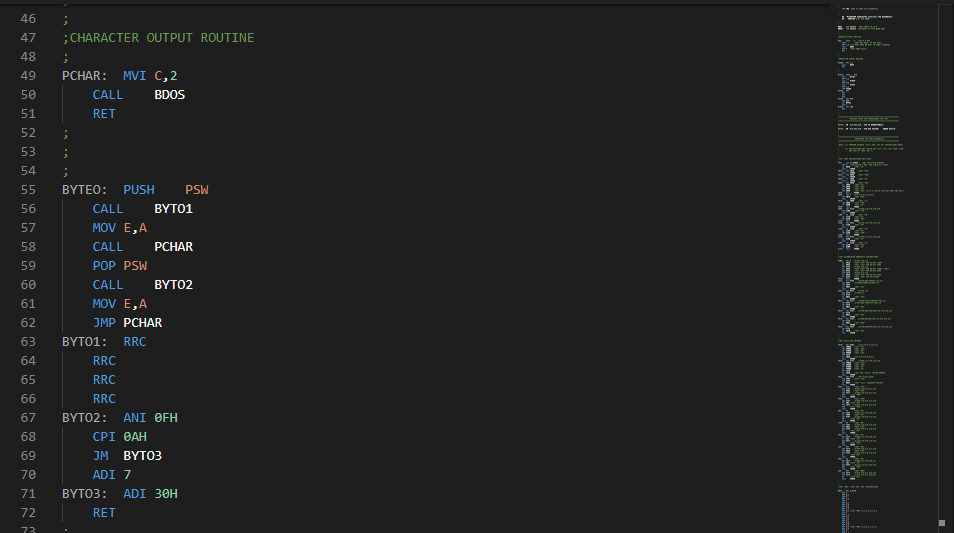
\includegraphics[width=1.0\textwidth]{Bilder/CodeEditor.png}
    \label{fig:codeeditor}
\end{figure}

In Abbildung \ref{fig:codeeditor} sieht man den Code-Editor in Aktion. Die einzelnen Bestandteile des Assembly-Codes, die Labels, die Instruktionen und die Argumente, sowie Kommentare sind alle unterschiedlich eingefärbt.

\begin{figure}
    \caption{Autovervollständigung für Instruktionen}
    \centering
    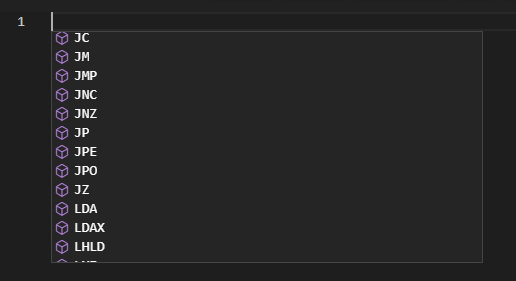
\includegraphics[width=0.6\textwidth]{Bilder/Completion1.png}
    \label{fig:completion1}
\end{figure}

In Abbildung \ref{fig:completion1} sieht man außerdem, wie die Autovervollständigung des Code-Editors funktioniert. Basierend auf der Eingabe des Nutzers und der Position im Code wird automatisch erkannt, ob eine Instruktion oder ein Argument vorgeschlagen werden soll und welche in Frage kommen.

\subsection{Emulator-Zustand}

Hat der Nutzer nun ein Assembly-Programm mithilfe des Code-Editors erstellt, kann er es ausführen. Hierfür wird der in Rust entwickelte Emulator genutzt, der mithilfe der \ac{WASM}-Schnittstelle in die Webapplikation eingebunden wird. Die Interaktion mit dem Emulator erfolgt mithilfe verschiedener Bedienelemente in einer Aktionsleiste am oberen Rand der Anwendung (siehe Abbildung \ref{fig:actionbar}).

\begin{figure}[h]
    \caption{Aktionsleiste des Emulators}
    \centering
    
\includegraphics[width=0.75\textwidth]{Bilder/Aktionsleiste.png}
    \label{fig:actionbar}
\end{figure}

\begin{figure}
    \caption{\textit{Load}-Dialog}
    \centering
    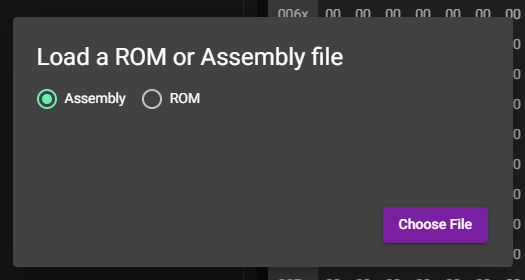
\includegraphics[width=0.75\textwidth]{Bilder/LoadDialog.png}
    \label{fig:loaddialog}
\end{figure}

Die ersten beiden Schaltflächen der Aktionsleiste, \textit{Load} und \textit{Save}, ermöglichen dem Nutzer, Assemblycode aus Dateien von seinem Endgerät zu laden oder sie dort zu speichern. \textit{Load} kann außerdem auch bereits übersetzten Code direkt in den Speicher des Emulators laden. Die Auswahl erfolgt mithilfe eines eigenen Auswahldialogs, der in Abbildung \ref{fig:loaddialog} zu sehen ist. Wird ein fertiges Programm geladen, kann außerdem bestimmt werden, an welcher Stelle es im Arbeitsspeicher platziert werden soll. Dies ist notwendig, da viele Programme beispielsweise erwarten, dass sich der Einstiegspunkt an der Speicheradresse 256 befindet.

Um den Code, den der Nutzer geschrieben hat, nun zu assemblen, muss dieser in der Aktionsleiste die Funktion \textit{Assemble} nutzen. Ist der Vorgang erfolgreich, werden die Bytes, die der Assembler erzeugt, in den Hauptspeicher des Emulators geschrieben. Die Emulation kann jetzt mithilfe der grünen Schaltfläche gestartet werden. Da die CPU keinen festgelegten Endzustand hat, läuft dieser solange weiter, bis der Nutzer die Emulation wieder beendet, was mit dem roten Stop-Knopf möglich ist.

Um den Ablauf des Codes nachvollziehen zu können, bietet die Applikation die Möglichkeit, jederzeit den internen Status des Prozessors einzusehen. Hierzu existiert auf der rechten Hälfte der Webseite eine Matrix, die den Arbeitsspeicher repräsentiert, sowie eine Anzeige für jedes der Register (siehe Abbildung \ref{fig:cpustate}).

\begin{figure}
    \caption{Anzeigen für den CPU-Status}
    \centering
    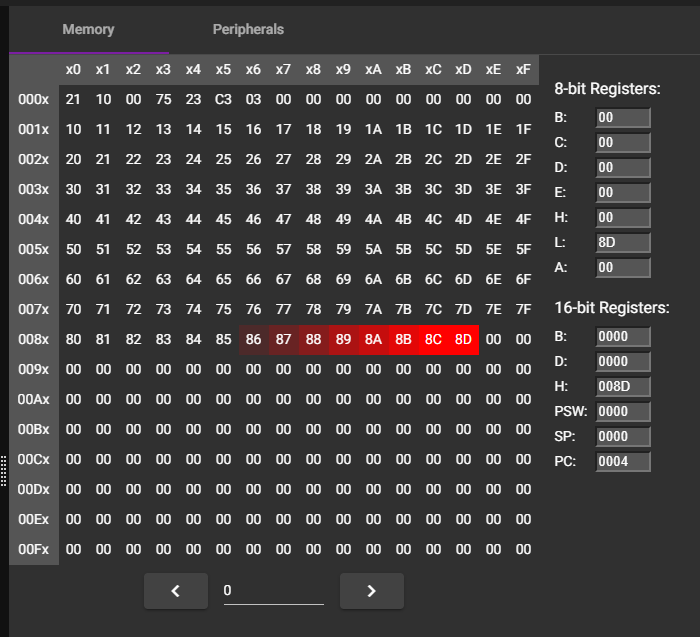
\includegraphics[width=0.75\textwidth]{Bilder/CPUState.png}
    \label{fig:cpustate}
\end{figure}

Die \ac{RAM}-Matrix stellt in jeder Zeile 16 Addressen dar, was die einfache Zuordnung von Zeile zu Spalte mithilfe der letzten Hexadezimalstelle erlaubt. Ändert sich im Arbeitsspeicher durch eine Instruktion des Prozessors ein Wert, wird dieser für eine kurze Zeit rot hinterlegt, um einfacher zu sehen, was sich geändert hat. Da der Speicher in der Regel deutlich größer ist, als die dargestellten 16x16 Bytes, nämlich bis zu 64KB, ist es möglich, den angezeigten Speicherbereich zu verschieben.

Die Registeranzeigen rechts von der \ac{RAM}-Matrix sind in zwei Kategorien gegliedert: Die 8-Bit Register (B, C, D, E, H, L, A) und die 16-Bit Register (BC, DE, HL, PSW, SP, PC).

Die aktuell ausgeführte Instruktion des Prozessors (basierend auf dem Program Counter) wird im Code-Editor außerdem rot hinterlegt. Für das Debugging von Programmen gibt es die Möglichkeit, die Ausführung des Emulators mithilfe der gelben Pause-Schaltfläche in der Aktionsleiste zu pausieren. Im pausierten Zustand kann nun jede Instruktion Schritt für Schritt ausgeführt werden.
\chapter{Implementierung}\label{chap:impl}

\section{Emulator}

\subsection{Registerarray}

Im folgenden werden drei Aspekte der Implementierungen des Registerarrays gezeigt: Die Repräsentation der Register, der Zugriff auf die Register und der Zugriff auf die Flaggen.

\subsubsection{Datentyp}

Naive Implementierungen eines Registerarrays würden die Register einzeln implementieren und für Registerpaare die entsprechenden Inhalte konkatenieren.
Dies ist jedoch unnötig umständlich. Der effizientere Ansatz ist die Register in Paaren zu speichern (als 16-Bit Unsigned Integer) und die Möglichkeit beizubehalten, die beiden Bytes individuell anzusprechen. In einer Sprache wie C ist dies mit Pointer-Arithmetik gut lösbar, in Rust ist es sinnvoller ein Union zu verwenden.

\begin{minted}{rust}
#[repr(C)]
union Register {
    bytes: (u8, u8),
    value: u16,
}
\end{minted}

Ein Union wird ähnlich wie ein Struct deklariert, jedoch teilen alle Felder den gleichen Speicherplatz\footnote{ausführliche Erklärung: \url{https://doc.rust-lang.org/reference/items/unions.html}}. Das bedeutet man kann den Wert eines solchen \rust{Register} entweder durch \rust{Register::bytes} als Tupel aus 2 Bytes oder durch \rust{Register::value} als 16-Bit-Wert auslesen. Dadurch ist keinerlei Konkatenation der Registerwerte notwendig.

\subsubsection{Registerzugriff}

Der Registerzugriff ist eine sehr häufig verwendete Operation, da ein großer Teil der zu implementierenden Instruktionen sie benötigt. Um dies möglichst einfach zu machen, wurde Indizierung für den Registerarray implementiert. Über String-Indizierung --- \rust{reg["bc"] // Registerpaar BC} --- ist Zugriff auf Registerpaare geregelt, über Character-Indizierung --- \rust{reg['b'] // Register B} --- der normale Zugriff.

\subsubsection{Flaggenzugriff}

Die Flags sind bekannterweise Teil des PSW-Registerpaars, sprich sie sind als einzelnes Byte gespeichert. Um die Werte der einzelnen Flaggen zu erhalten, werden Bitmasken verwendet. Um bspw. herauszufinden, ob das Bit mit dem höchsten Stellenwert gesetzt ist, muss der Ausdruck \rust{byte & 0x80 != 0} berechnet werden. Wenn dieser \rust{true} ist, ist das Bit gesetzt\footnote{\rust{0x80 == 0b10000000}}.

\subsection{Ein-/Ausgabegeräte}

In \cref{chap:design} ist zu sehen, dass die zentrale Struktur 2 Arrays mit 256 Elementen beinhaltet, um Ein- und Ausgabegeräte zu realisieren. Der Datentyp dieser Arrays wurde jedoch, der Übersichtlichkeit halber, vereinfacht. Das erste Problem eines solchen Arrays ist, dass initial keine Geräte registriert sind. Da es in Rust kein \rust{null} gibt, wäre das schlecht umsetzbar. Daher muss der \rust{Option}-Typ verwendet werden:

\rust{[Option<InputDevice>; 256]}

Hier ist jetzt jedoch problematisch, dass verschiedene Geräte registriert werden können. In klassischen objektorientierten Sprachen, wären Input- bzw OutputDevice hier Interfaces, in Rust arbeiten wir mit Traits (siehe \cref{chap:prereqs}). Da die Größe von Trait-Objekten nicht zur Compilezeit bestimmt werden kann, kann ein solches Objekt nicht auf dem Stack gelagert werden, daher muss ein Pointer verwendet werden. Rust verwendet sogenannte Smartpointer um die klassischen Probleme bei Verwendung von Pointern zu vermeiden. Meistens verwendet man hier \rust{Box}, jedoch erlaubt Box nicht, mehrere Referenzen auf die Daten zu haben. Dies brauchen wir jedoch, da sowohl von außen, als auch von innen mit den Geräten kommuniziert werden muss. Durch Kombination von \rust{Rc}, einem referenzzählendem Pointer, mit \rust{RefCell}, einer schreibbaren Speicherregion, kann das gewollte Verhalten erreicht werden. Die Syntax um einen derartigen Array zu deklarieren ist wie folgt:

\rust{[Option<Rc<RefCell<dyn InputDevice>>>; 256]}

Solange unser Programm single-threaded ist, kann nun jederzeit eine mutable-Referenz auf ein solches InputDevice erhalten werden und solange im aktuellen Scope keine mutable Referenz auf das Gerät existiert, können beliebig viele non-mutable Referenzen verwendet werden.

\chapter{Auswertung}\label{chap:eval}

\section{Testprogramme}

Ziel dieser Arbeit ist es, die komplette Spezifikation des Intel 8080 zu implementieren. Um zu überprüfen, ob dies tatsächlich gelungen ist, müssen Tests durchgeführt werden. Hierfür kommen frei verfügbare \footnote[1]{\url{https://altairclone.com/downloads/cpu_tests/}} CPU Testprogramme zum Einsatz, die die Funktionsweise verschiedener Instruktionen überprüfen und mit Sollzuständen vergleichen.



\end{document}
